\documentclass{article}
\usepackage{fullpage}
\usepackage{graphicx}
\graphicspath{{../images-videos/}}  
\usepackage{titlesec}
\usepackage{amsmath}
\usepackage{amssymb}
\usepackage{array}
\usepackage{float}
\usepackage{xcolor}
\renewcommand{\baselinestretch}{2}
\usepackage{hyperref}  % Optional for clickable ToC
\usepackage{ulem} 
\author{Paradiso Emiliano,  \quad 1940454 \\Vittorio Pisapia,  \quad 1918590 \\Brian Piccione, \quad da scrivere}
\title{\Huge Medical Robotics project \\ \centering \Large \textbf{Shared control of a teleoperated echographic probe}}

\hypersetup{
    colorlinks=true,            % Collega con colori invece che riquadri
    urlcolor=blue,              % Colore dei collegamenti ipertestuali
    linkcolor=black 
}

\titleformat{\chapter}[block]
  {\normalfont\LARGE\bfseries} 
  {}                           
  {0pt}                      
  {\LARGE}              

\begin{document}
\maketitle
\vspace{2cm}

\begin{abstract}
%% SCRIVI L'ABSTRACT
\hspace*{-0.5cm}In this work, we aim to design a robust control law for tracking a periodic joint space trajectory for a 3R spatial manipulator, based on bounds on its dynamic coefficients. To achieve this, we will derive the dynamic model and extract a linear parameterization in terms of a minimal set of dynamic coefficients. We will then apply robust control theory to the case in exam. Additionally, we will conduct simulations to evaluate the performance of our designed control law, highlighting the main benefits of robust control in contrast to a classic control law such as feedback linearization under both ideal and uncertain conditions.
\\GitHub link: \uline{\href{https://github.com/VittorioPisapia/Medical-Robotics/tree/main}{Project GitHub}}
\end{abstract}

\newpage
\tableofcontents
\newpage

\section{Problem introduction}

\section{State of the art}
In this chapter, we will examine various works and systems related to tele-echography. Our focus will be on providing detailed descriptions of four specific systems. Additionally, we will mention other systems such as MIDSTEP, RUDS, SYRTECH, TERESA, and ESTELE.

\subsection{The TER system}
Among the various tele-ultrasound systems, TER is a tele-robotic system consisting of a master workstation (with or without force feedback control) and a slave robot operated remotely by a clinician to perform ultrasound-based diagnoses. The master system has been developed and tested with two approaches: one using a position sensor with visual feedback, and another incorporating a haptic device for force feedback. A unique feature of TER is its slave system, which is actuated by artificial muscles, giving it natural compliance.

\begin{figure}[h]
    \centering
    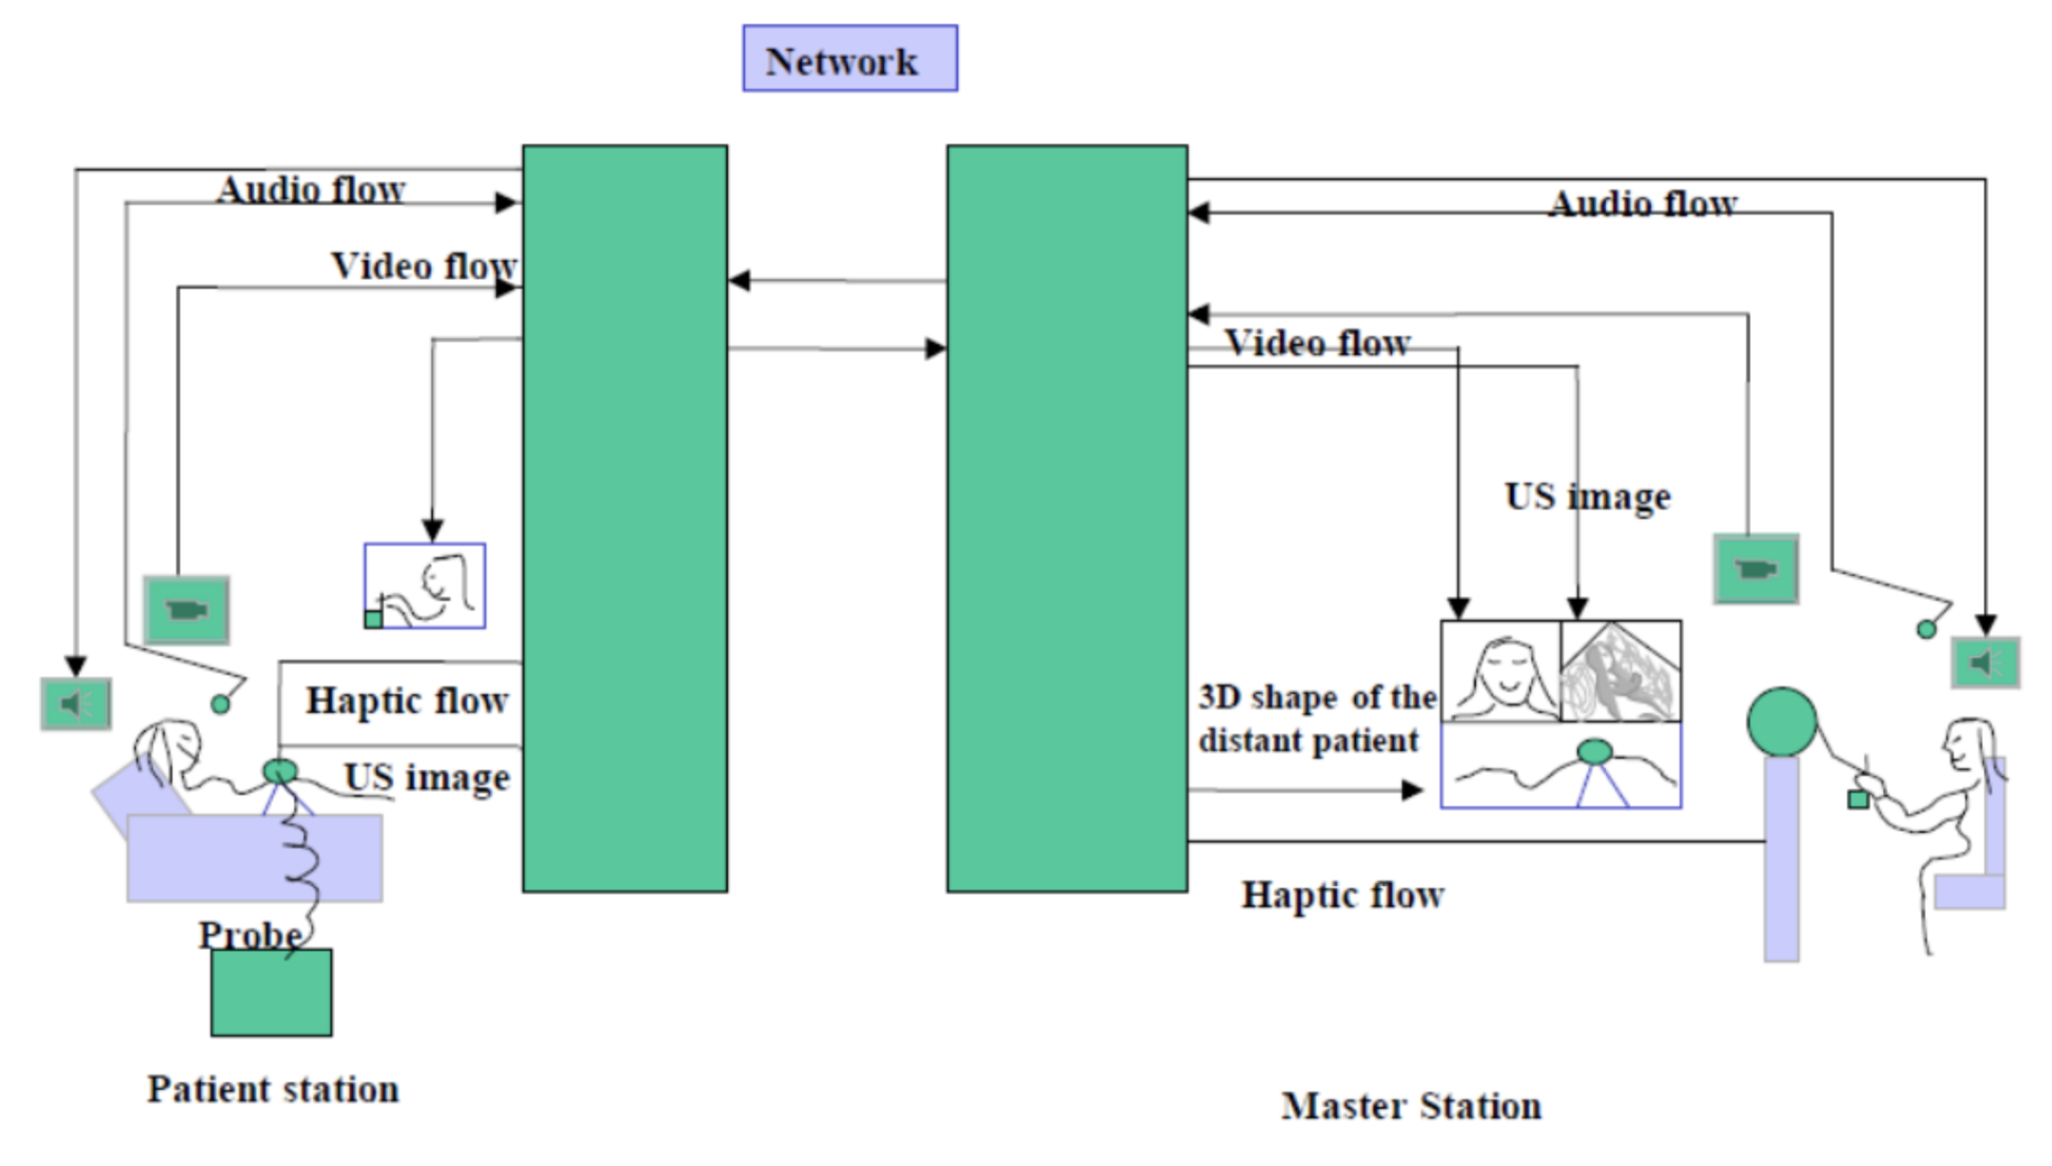
\includegraphics[width=0.5\textwidth]{TER.png}  
    \caption{TER architecture}
    \label{fig:ter}
\end{figure}


\section{Development}

\section{Conclusion}

\section{Future works}



\addcontentsline{toc}{section}{References}
\begin{thebibliography}{9}

\bibitem{Spong}
  M. Spong,
  \emph{“On the robust control of robot manipulators”},
   IEEE Trans . on Automatic Control, 37(11), 1782-1786, 1992.

\bibitem{Slotine}
  J.-J. E. Slotine, and W. Li,
  \emph{“On the adaptive control of robot manipulators”},
  Int. J. Robot. Research, vol. 6, no. 3, pp. 49-59, Fall 1987.
   
\bibitem{De Luca}
  A. De Luca,
  \emph{RobustControl},
 Block of slides 11 RobustControl of Robotics 2

\end{thebibliography}

\end{document}